
\begin{center}
\thispagestyle{empty}


\vspace{.5cm}

%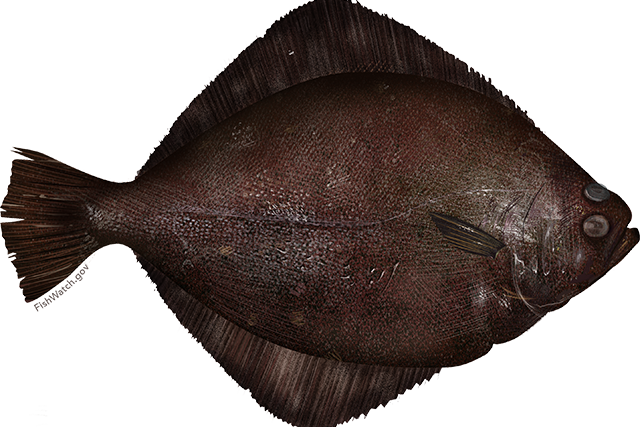
\includegraphics{petrale_sole}~\\[0.5cm]
%\pdftooltip{\includegraphics{Sebastes_alutus}}{This is a fish.}



Chantel R. Wetzel\textsuperscript{1}\\


\vspace{.5cm}

\small
\textsuperscript{1}Northwest Fisheries Science Center, U.S. Department of Commerce, National Oceanic and Atmospheric Administration, National Marine Fisheries Service, 2725 Montlake Boulevard East, Seattle, Washington 98112\\

\vspace{.3cm}





\vspace{1cm}

\vfill
October 2019

\vspace{1cm}

%DRAFT SAFE\\
%Disclaimer: This information is distributed solely for the purpose of pre-dissemination
%peer review under applicable information quality guidelines. It has not been formally
%disseminated by NOAA Fisheries. It does not represent and should not be construed to
%represent any agency determination or policy. 


\vspace{.3cm}
%Bottom of the page
%{\large \today}

\newpage

\vspace{3cm}

This report may be cited as:\\

Wetzel, C.R. 2019. Status of petrale sole (\textit{Eopsetta jordani}) along the U.S. west coast in 2019. Pacific Fishery Management Council, 7700 Ambassador Place NE, Suite 101, Portland, OR 97220. 
\end{center}

\vspace{3cm}



\maketitle


\pagenumbering{roman}
\setcounter{page}{1}



